\PassOptionsToPackage{dvipsnames,svgnames,x11names}{xcolor}
\documentclass[landscape,a0paper,fontscale=0.35]{baposter}



% For graphs
\usepackage{graphicx}
\usepackage{array}
\usepackage{booktabs}
\usepackage{eso-pic}
\usepackage{layout}
\usepackage{fancybox}
\usepackage{calc}
\usepackage{amsmath}
\usepackage{amssymb}
\usepackage{relsize}
\usepackage{multirow}
\usepackage{rotating}
\usepackage{bm}
\usepackage{url}
\usepackage{xfrac}
\usepackage{natbib}
\setcitestyle{round}
\usepackage{mathtools}
\usepackage{cancel}
\usepackage{paralist}
\usepackage{nicefrac}
\usepackage[export]{adjustbox} % loads also graphicx
\usepackage{caption}
\usepackage{xfrac}
\usepackage{multicol}
\newcommand{\figurewidth}{7cm}
\newcommand{\figureheight}{3cm}
\usepackage{palatino}
\usetikzlibrary{calc}
\usepackage{mymacros}
\usepackage{mathabx}
\usepackage{multicol}
\usepackage{enumitem}
\usepackage{array}
\newcolumntype{L}[1]{>{\raggedright\let\newline\\\arraybackslash\hspace{0pt}}m{#1}}
\newcolumntype{C}[1]{>{\centering\let\newline\\\arraybackslash\hspace{0pt}}m{#1}}
\newcolumntype{R}[1]{>{\raggedleft\let\newline\\\arraybackslash\hspace{0pt}}m{#1}}


\renewcommand{\sfdefault}{lmss}
\sffamily

\newcommand{\listhead}[1] {\textsc{\underline{#1}}}

\usepackage{tikz,pgfplots}
\pgfplotsset{compat=newest}
\tikzstyle{every picture}+=[remember picture]
\tikzstyle{na} = [baseline=-.5ex]
\everymath{\displaystyle}
\usetikzlibrary{arrows,shapes}
\usetikzlibrary{positioning}

\usepackage{wasysym}

\usepackage{algorithm}
\usepackage{algorithmic}

\usepackage{multirow}

\usepackage{tabu}

\usepackage{xspace}
\DeclareRobustCommand{\eg}{e.g.,\@\xspace}
\DeclareRobustCommand{\ie}{i.e.,\@\xspace}
\DeclareRobustCommand{\wrt}{w.r.t.\@\xspace}
\DeclareRobustCommand{\wp}{w.p.\@\xspace}

\usepackage{bm}
\newcommand{\mathbr}[1]{\bm{\mathbf{#1}}}

\usepackage{lettrine}
\usepackage{xspace}

%=============================================
% General commands
%---------------------------------------------

%=============================================
%%Custom commands

%Colors
\definecolor{darkcyan}{rgb}{0.0, 0.55, 0.55}
\definecolor{darkcerulean}{rgb}{0.03, 0.27, 0.49}
\definecolor{crimson}{rgb}{0.86, 0.08, 0.24}
\definecolor{limegreen}{rgb}{0.2, 0.8, 0.2}
\colorlet{fcolor}{darkcerulean}
\colorlet{errcolor}{darkcyan}
\definecolor{projcolor}{named}{black}
\colorlet{dotcolor}{fcolor}
\colorlet{boundcolor}{violet}
\definecolor{newdotcolor}{named}{green}
\definecolor{arrowcolor}{named}{blue}
\definecolor{distcolor}{rgb}{0.36, 0.11, 0.63}
\definecolor{poliblue1}{RGB}{93,138,168} 
\definecolor{poliblue2}{RGB}{41,76,113}
\definecolor{poliblue3}{RGB}{25,43,67}
\definecolor{orangep}{RGB}{251,146,116}

\usetikzlibrary{tikzmark}

%Decorations
\newcommand{\bad}[1]{\textcolor{crimson}{\textbf{#1}}}
\newcommand{\good}[1]{\textcolor{limegreen}{\textbf{#1}}}

\newcommand{\enb}[1]{\textcolor{poliblue1}{\textbf{#1}}}
\newcommand{\eno}[1]{\textcolor{orangep}{\textbf{#1}}}

%Fake items
\newcommand{\tabitem}[1]{~~\llap{\textbullet}~~ #1 \hfill\mbox{}}

%%%%%%%%%%%%%%%%%%%%%%%%%%%%%%%%%%%%%%%%%%%%%%%%%%%%%%%%%%%%%%%%%%%%%%%%%%%%%%%%
%%%% Some math symbols used in the text
%%%%%%%%%%%%%%%%%%%%%%%%%%%%%%%%%%%%%%%%%%%%%%%%%%%%%%%%%%%%%%%%%%%%%%%%%%%%%%%%

%%%%%%%%%%%%%%%%%%%%%%%%%%%%%%%%%%%%%%%%%%%%%%%%%%%%%%%%%%%%%%%%%%%%%%%%%%%%%%%%
% Multicol Settings
%%%%%%%%%%%%%%%%%%%%%%%%%%%%%%%%%%%%%%%%%%%%%%%%%%%%%%%%%%%%%%%%%%%%%%%%%%%%%%%%
\setlength{\columnsep}{1.5em}
\setlength{\columnseprule}{0mm}

%%%%%%%%%%%%%%%%%%%%%%%%%%%%%%%%%%%%%%%%%%%%%%%%%%%%%%%%%%%%%%%%%%%%%%%%%%%%%%%%
% Save space in lists. Use this after the opening of the list
%%%%%%%%%%%%%%%%%%%%%%%%%%%%%%%%%%%%%%%%%%%%%%%%%%%%%%%%%%%%%%%%%%%%%%%%%%%%%%%%
\newcommand{\compresslist}{%
\setlength{\itemsep}{1pt}%
\setlength{\parskip}{0pt}%
\setlength{\parsep}{0pt}%
}

\newcommand{\mildcompresslist}{%
\setlength{\itemsep}{2pt}%
\setlength{\parskip}{1pt}%
\setlength{\parsep}{1pt}%
}

\captionsetup{justification=raggedright,singlelinecheck=false}

%Reduce linespace in biblio
\setlength{\bibsep}{1.5pt}

\usepackage[many]{tcolorbox}
\usetikzlibrary{decorations.pathreplacing}
\usetikzlibrary{backgrounds}

\usepackage{stackengine}
\usepackage{scalerel}
\newcommand\dangersign[1][2ex]{%
	\renewcommand\stacktype{L}%
	\scaleto{\stackon[1.5pt]{\color{crimson}$\triangle$}{\tiny \bfseries{!}}}{#1}%
}

\definecolor{amethyst}{rgb}{0.6, 0.4, 0.8}
%\newcommand{\firstletter}[1]{{\fcolorbox{black}{black}{\scalebox{2}{\fontsize{24pt}{0pt}\selectfont \textcolor{white}{\textbf{#1}}}}}}

%Transparent boxes
\makeatletter 
\renewcommand{\baposter@box@drawbackground@plain}[2]{\tikzset{box colors/.style={fill=#1,fill opacity=1}} \fill[box colors] \baposterBoxGetShape;}
\makeatother


%%%%%%%%%%%%%%%%%%%%%%%%%%%%%%%%%%%%%%%%%%%%%%%%%%%%%%%%%%%%%%%%%%%%%%%%%%%%%%
%%% Begin of Document
%%%%%%%%%%%%%%%%%%%%%%%%%%%%%%%%%%%%%%%%%%%%%%%%%%%%%%%%%%%%%%%%%%%%%%%%%%%%%%

\begin{document}

%%%%%%%%%%%%%%%%%%%%%%%%%%%%%%%%%%%%%%%%%%%%%%%%%%%%%%%%%%%%%%%%%%%%%%%%%%%%%%
%%% Here starts the poster
%%%---------------------------------------------------------------------------
%%% Format it to your taste with the options
%%%%%%%%%%%%%%%%%%%%%%%%%%%%%%%%%%%%%%%%%%%%%%%%%%%%%%%%%%%%%%%%%%%%%%%%%%%%%%

\background{%
}


% Define some colors
\definecolor{blue900}{HTML}{0D47A1}
\definecolor{blue800}{HTML}{1565C0}
\definecolor{lightblue}{rgb}{0.145,0.6666,1}

% \begin{tikzpicture}
%  	\pgfmathsetseed{100000}
%  	\foreach \i in {1,...,300}
%		\node[circle,draw=none,fill=violet!15,minimum size=50 + rand * 30]
%        () at (rand * \paperwidth + \paperwidth, rand * \paperheight + \paperheight) {};
%  \end{tikzpicture}

\begin{poster}%
  % Poster Options
  {
  % Show grid to help with alignment
  columns=4,
  grid=false,
  % Column spacing
  colspacing=1em,
  % Color style
  bgColorOne=white,
  bgColorTwo=white,
  borderColor=blue900,
  headerColorOne=blue800,
  headerColorTwo=blue800,
  headerFontColor=white,
  boxColorOne=white,
  boxColorTwo=lightblue,
  % Format of textbox
  textborder=roundedleft,
  % Format of text header
  eyecatcher=true,
  headerborder=closed,
  headerheight=0.095\textheight,
%  textfont=\sc, An example of changing the text font
  headershape=roundedright,
  headershade=shadelr,
  headerfont=\large\bf\textsc, %Sans Serif
  textfont={\setlength{\parindent}{1.5em}},
  boxshade=plain,
%  background=shade-tb,
  background=user,
  linewidth=2pt
  }
  % Eye Catcher
  % {
\includegraphics[height=9em]{./pics/airlab_logo_reflect.png}} 
  {\hspace{0.5cm} 
\includegraphics[height=7.0em]{./pics/polilogo/logoPoliBlue_poster.png} \hspace{2cm}}
%   {\hspace{3.5cm}}
  % Title
  {\bf\textsc{Optimistic Policy Optimization via Multiple Importance Sampling}\vspace{0.1em}}
  % Authors
  {\textsc{Matteo Papini, Alberto M. Metelli, Lorenzo Lupo and Marcello Restelli}\\ 
  {\normalsize \texttt{\{matteo.papini, albertomaria.metelli, marcello.restelli\}@polimi.it, lorenzo.lupo@mail.polimi.it}}
  }
  % University logo
  {% The makebox allows the title to flow into the logo, this is a hack because of the L shaped logo.
    %
\includegraphics[height=9.0em]{./pics/PoliMI.pdf}%\hspace{.5cm}
    {
\includegraphics[height=7.0em]{../talk/qr.png}}
  }
%%%%%%%%%%%%%%%%%%%%%%%%%%%%%%%%%%%%%%%%%%%%%%%%%%%%%%%%%%%%%%%%%%%%%%%%%%%%%%
%%% Now define the boxes that make up the poster
%%%---------------------------------------------------------------------------
%%% Each box has a name and can be placed absolutely or relatively.
%%% The only inconvenience is that you can only specify a relative position 
%%% towards an already declared box. So if you have a box attached to the 
%%% bottom, one to the top and a third one which should be in between, you 
%%% have to specify the top and bottom boxes before you specify the middle 
%%% box.
%%%%%%%%%%%%%%%%%%%%%%%%%%%%%%%%%%%%%%%%%%%%%%%%%%%%%%%%%%%%%%%%%%%%%%%%%%%%%%

%%%%%%%%%%%%%%%%%%%%%%%%%%%%%%%%%%%%%%%%%%%%%%%%%%%%%%%%%%%%%%%%%%%%%%%%%%%%%%
\headerbox{Motivation and Idea}{name=problem,column=0,row=0,span=1}{
	%%%%%%%%%%%%%%%%%%%%%%%%%%%%%%%%%%%%%%%%%%%%%%%%%%%%%%%%%%%%%%%%%%%%%%%%%%%%%%
	\noindent\:\bad{Problem}
	\begin{itemize}
	\compresslist
		\item \textbf{Policy Optimization (PO)} methods \eno{neglect exploration}
		\item Existing exploration strategies are \eno{undirected}
		\item Lack of \enb{provably efficient} solutions
	\end{itemize}

	\noindent\:\good{Idea}
	\begin{itemize}
	\compresslist
		\item Frame PO as a continuous \textbf{Multi-Armed Bandit (MAB)}
		\item Use \textbf{Multiple Importance Sampling (MIS)} to exploit natural \textbf{arm correlation}
		\item Apply \textbf{Optimism in Face of Uncertainty (OFU)}
	\end{itemize}
}

%%%%%%%%%%%%%%%%%%%%%%%%%%%%%%%%%%%%%%%%%%%%%%%%%%%%%%%%%%%%%%%%%%%%%%%%%%%%%%

%%%%%%%%%%%%%%%%%%%%%%%%%%%%%%%%%%%%%%%%%%%%%%%%%%%%%%%%%%%%%%%%%%%%%%%%%%%%%%
\headerbox{Policy Optimization}{name=polopt,column=0,row=1,span=1, below=problem}{
	%%%%%%%%%%%%%%%%%%%%%%%%%%%%%%%%%%%%%%%%%%%%%%%%%%%%%%%%%%%%%%%%%%%%%%%%%%%%%%
	\begin{itemize}
	\compresslist
		\item \eno{Continuous} MDP $\left\langle\Sspace,\Aspace,\Tran,\Rew,\gamma,\init\right\rangle$
		\item \textbf{Trajectories} $\tau = s_0, a_0, r_1, s_1, \dots r_H \quad\in\quad \mathcal{T}$
		\item Return $\Rew(\tau) = \sum_{h=0}^{H-1}\gamma^h r_{h+1}$
	\end{itemize}
	\centering
	
	\tikzstyle{background rectangle}=[thick, draw=blue!50]
	\noindent \begin{tikzpicture}[show background rectangle]
		\node[align=justify, text width=0.9\textwidth, inner sep=0.8em]{
		\vspace{-0.65cm}
	\begin{center}
	\citep{peters2008reinforcement}
	\noindent\begin{minipage}[t]{0.52\linewidth}
		\hspace{-0.2cm}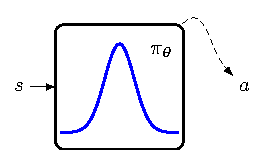
\includegraphics[scale=0.9]{ab}
	\end{minipage}%
	\noindent\begin{minipage}[t]{0.48\linewidth}
	\vspace{-2cm}
	%\begin{itemize}[leftmargin=*]
	%\compresslist
		\centerline{\enb{Parametric Policy}}\vspace{-0.4cm}
		$$\pi_{\vtheta} \text{ with }\vtheta\in\Theta$$
	\begin{itemize}[leftmargin=*]
		\item Induced \textbf{trajectory distribution} $p_{\vtheta}(\tau)$
	\end{itemize}
	\end{minipage}
	$$\vtheta^*=\arg\max_{\vtheta\in\Theta} J(\vtheta)\coloneqq \mathbb{E}_{\tau\sim p_{\vtheta}}[\Rew(\tau)]$$
	\end{center}
%	\begin{itemize}[leftmargin=*]
%	\mildcompresslist
%		\item \enb{Parametric Policy} $\pi_{\vtheta}:\Sspace\to\Aspace$ with $\vtheta\in\Theta$
%		\item Induced \textbf{trajectory distribution} $p_{\vtheta}(\tau)$
%		%\item \textbf{Performance} $J(\vtheta) = \mathbb{E}_{\tau\sim p_{\vtheta}}[\Rew(\tau)]$
%		\item Find 
%	\end{itemize}
%	
%	\begin{minipage}[t]{0.65\linewidth}
%	\begin{itemize}[leftmargin=*]
%	\mildcompresslist
%		\item \enb{Parametric Policy} $\pi_{\vtheta}:\Sspace\to\Aspace$ with $\vtheta\in\Theta$
%		\item Induced \textbf{trajectory distribution} $p_{\vtheta}(\tau)$
%		%\item \textbf{Performance} $J(\vtheta) = \mathbb{E}_{\tau\sim p_{\vtheta}}[\Rew(\tau)]$
%		\item Find $\vtheta^*=\arg\max_{\vtheta\in\Theta} J(\vtheta)\coloneqq \mathbb{E}_{\tau\sim p_{\vtheta}}[\Rew(\tau)]$
%	\end{itemize}
%	\end{minipage}%
%	\hfill
%	\begin{minipage}[t]{0.34\linewidth}
%		
%	\end{minipage}	
	};
	\node[overlay, fill=white, draw=white, above] at (current bounding box.north) {\textcolor{blue}{\textbf{Action-based PO}}};
	\end{tikzpicture} \\
	\vspace{0.2cm}
	\tikzstyle{background rectangle}=[thick, draw=red!50]
	\noindent \begin{tikzpicture}[show background rectangle]
		\node[align=justify, text width=0.9\textwidth, inner sep=0.8em]{
		\vspace{-0.65cm}
	\begin{center}
	\citep{sehnke2008policy}\\
	\vspace{-0.2cm}
	\noindent\begin{minipage}[t]{0.52\linewidth}
		\hspace{-0.2cm}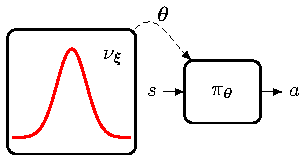
\includegraphics[scale=0.9]{pb}
	\end{minipage}%
	\noindent\begin{minipage}[t]{0.48\linewidth}
	\vspace{0.5cm}
	%\begin{itemize}[leftmargin=*]
	%\compresslist
		\centerline{\enb{Parametric Hyperpolicy}}\vspace{-0.4cm}
		$$\nu_{\vxi} \text{ with } \vxi\in\Xi$$
	%\end{itemize}
	\end{minipage}
	$$\vxi^* = \arg\max_{\vxi\in\Xi}J(\vxi) \coloneqq \mathbb{E}_{\vtheta\sim\nu_{\vxi}}\left[J(\vtheta)\right]$$
	\end{center}};
	\node[overlay, fill=white, draw=white, above] at (current bounding box.north) {\textcolor{red}{\textbf{Parameter-based PO}}};
	\end{tikzpicture}	
%	\noindent\: \textcolor{blue}{\textbf{Action-based PO}}\\ \citep{peters2008reinforcement}
%	%\centerline{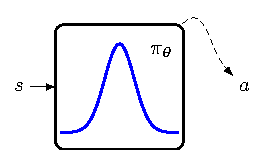
\includegraphics[scale=1]{ab}}
%	\begin{itemize}
%	\mildcompresslist
%		\item \enb{Parametric Policy} $\pi_{\vtheta}:\Sspace\to\Aspace$ with $\vtheta\in\Theta$ (\eg Gaussian)
%		\item Induced \textbf{trajectory distribution} $p_{\vtheta}(\tau)$
%		%\item \textbf{Performance} $J(\vtheta) = \mathbb{E}_{\tau\sim p_{\vtheta}}[\Rew(\tau)]$
%		\item Find $\vtheta^*=\arg\max_{\vtheta\in\Theta} J(\vtheta)\coloneqq \mathbb{E}_{\tau\sim p_{\vtheta}}[\Rew(\tau)]$
%	\end{itemize}
%	\centering
%\noindent\: \textcolor{red}{\textbf{Parameter-based PO}}\\ \citep{sehnke2008policy}
%%\centerline{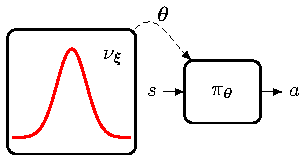
\includegraphics[scale=1]{pb}}
%\begin{itemize}
%\mildcompresslist
%	\item \enb{Parametric Hyperpolicy} $\nu_{\vxi}(\vtheta)$ with $\vxi\in\Xi$ (\eg Gaussian)
%	\item Find $\vxi^* = \arg\max_{\vxi\in\Xi}J(\vxi) \coloneqq \mathbb{E}_{\vtheta\sim\nu_{\vxi}}\left[J(\vtheta)\right]$
%\end{itemize}
\vspace{-0.4cm}
}

%%%%%%%%%%%%%%%%%%%%%%%%%%%%%%%%%%%%%%%%%%%%%%%%%%%%%%%%%%%%%%%%%%%%%%%%%%%%%%

%%%%%%%%%%%%%%%%%%%%%%%%%%%%%%%%%%%%%%%%%%%%%%%%%%%%%%%%%%%%%%%%%%%%%%%%%%%%%%
\headerbox{Policy Optimization as Correlated MAB}{name=ucb,column=0,row=2,span=1, above=bottom}{
	%%%%%%%%%%%%%%%%%%%%%%%%%%%%%%%%%%%%%%%%%%%%%%%%%%%%%%%%%%%%%%%%%%%%%%%%%%%%%%
	\begin{itemize}
	\compresslist
		\item (Hyper)parameters as arms $\implies$ \eno{continuous} MAB
		\item Arms \enb{correlate} through common outcome space
	\end{itemize}
		\begin{minipage}{.45\textwidth}
			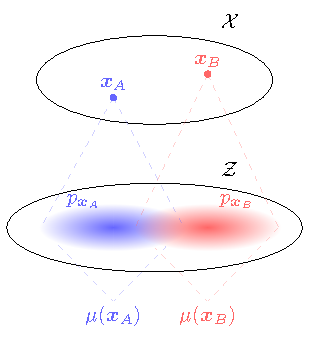
\includegraphics[width=\textwidth]{plots/spaces7.pdf}
		\end{minipage}\hfill%
		\begin{minipage}{.54\textwidth}
		\noindent\: MAB jargon:
		\begin{itemize}
			\item $\vx^* \in \arg\max_{\vx\in\Xspace} \mu(\vx)$
			\item Gap $\Delta_t = \mu(\vx^*) - \mu(\vx_t)$
			\item $\mathop{Regret}(T) = \sum_{t=0}^{T}\Delta_t$
		\end{itemize}
		\end{minipage}
}

%%%%%%%%%%%%%%%%%%%%%%%%%%%%%%%%%%%%%%%%%%%%%%%%%%%%%%%%%%%%%%%%%%%%%%%%%%%%%%

%%%%%%%%%%%%%%%%%%%%%%%%%%%%%%%%%%%%%%%%%%%%%%%%%%%%%%%%%%%%%%%%%%%%%%%%%%%%%%
\headerbox{Multiple Importance Sampling (MIS)}{name=mis,column=1,row=0,span=1}{
	%%%%%%%%%%%%%%%%%%%%%%%%%%%%%%%%%%%%%%%%%%%%%%%%%%%%%%%%%%%%%%%%%%%%%%%%%%%%%%
	\begin{itemize}
	\compresslist
		\item Samples from several \textbf{behavioral} distributions:\\ 
		$z_0 \sim q_0, z_1 \sim q_1, \dots, z_K \sim q_K$
%		\item \textbf{Target distribution} $p$
		\item Estimate $\mu\coloneqq\mathbb{E}_{z\sim p}\left[f(z)\right]$ under \textbf{target} distribution $p$
%		\item \textbf{Mixture} of behaviorals: $\vphi(z) = \frac{1}{K}\sum_{k=1}^K q_k(z)$
		\item \enb{Balance Heuristic (BH)}~\citep{veach_optimally_1995}:
		\begin{align*}
		&\wh{\mu}_{\text{BH}} \coloneqq \frac{1}{K}\sum_{k=1}^K\underbrace{\frac{p(z_{k})}{\Phi(z_k)}}_{\mathclap{\text{Importance Weight (IW)}}}f(z_{k}),
		&\qquad\underbrace{\Phi(z) = \frac{1}{K}\sum_{k=1}^K q_k(z)}_{\text{mixture}}
		\end{align*}
%		\item Unbiased: $\mathbb{E}[\wh{\mu}_{\text{BH}}] = \mu$
		\item \enb{Unbiased}, but possibly \eno{high-variance}:
			\begin{align*}
				&\Var\left[\wh{\mu}_{\text{BH}}\right] \leq \norm[\infty]{f}^2\frac{d_2(P\|\Phi)}{K} \leq 
				\norm[\infty]{f}^2\frac{1} {\sum_{k=1}^K \frac{1}{ d_{2}(p \| q_k)}} \\
				&\quad d_{2}(p\|q) \coloneqq \int_{\mathcal{Z}}\left(\frac{p(z)}{q(z)}\right)^{2}\de z \qquad \text{(R\'enyi divergence)}
			\end{align*}
	\end{itemize}
}

%%%%%%%%%%%%%%%%%%%%%%%%%%%%%%%%%%%%%%%%%%%%%%%%%%%%%%%%%%%%%%%%%%%%%%%%%%%%%%


%%%%%%%%%%%%%%%%%%%%%%%%%%%%%%%%%%%%%%%%%%%%%%%%%%%%%%%%%%%%%%%%%%%%%%%%%%%%%%
\headerbox{Robust MIS Estimator}{name=robust,column=2,row=0,span=1, bottomaligned=mis}{
	%%%%%%%%%%%%%%%%%%%%%%%%%%%%%%%%%%%%%%%%%%%%%%%%%%%%%%%%%%%%%%%%%%%%%%%%%%%%%%
	\begin{itemize}
	\compresslist
		\item Importance Sampling estimators are \eno{heavy-tailed}~\citep{metelli2018policy}
		\item This prevents the formation of \emph{exponential} \textbf{Upper Confidence Bounds (UCB)}
		\item Robust estimation via \enb{adaptive truncation}~\citep{bubeck2013bandits}:
		\vspace*{-.25cm}
		\begin{align*}\label{eq:truncatedmise}
			&\widecheck{\mu}_{\text{BH}} \coloneqq \frac{1}{K} \sum_{k=1}^K\min \left\{\underbrace{\sqrt{\frac{K d_{2}\left( p \| \Phi  \right)}{\log \frac{1}{\delta}}}}_{\mathclap{\text{truncation}}},  \underbrace{\vphantom{\sqrt{\frac{K d_{2}\left( p \| \Phi  \right)}{\log \frac{1}{\delta}}}}\frac{p(z_{k})}{\Phi(z_k)}}_{\text{IW}} \right\} f(z_{k})
		\end{align*}
		\item Thanks to truncation, with probability at least $1-2\delta$:
		\begin{align*}
			\left|\widecheck{\mu}_{\text{BH}} - \mu\right| \leq \|f\|_{\infty} \left(\sqrt{2} + \frac{4}{3} \right)  \sqrt{\frac{ d_{2}\left( p \| \Phi  \right) \log  \frac{1}{\delta}  }{K}}
		\end{align*}
	\end{itemize}
}

%%%%%%%%%%%%%%%%%%%%%%%%%%%%%%%%%%%%%%%%%%%%%%%%%%%%%%%%%%%%%%%%%%%%%%%%%%%%%%

%%%%%%%%%%%%%%%%%%%%%%%%%%%%%%%%%%%%%%%%%%%%%%%%%%%%%%%%%%%%%%%%%%%%%%%%%%%%%%
\headerbox{OPTIMIST Algorithm}{name=ucb,column=1,row=1,span=2, below=robust}{
	%%%%%%%%%%%%%%%%%%%%%%%%%%%%%%%%%%%%%%%%%%%%%%%%%%%%%%%%%%%%%%%%%%%%%%%%%%%%%%
\noindent \:A \textbf{UCB}-like algorithm based on the \textbf{Optimism in Face of Uncertainty} principle:
\begin{itemize}
\compresslist
	\item Select \emph{confidence schedule $(\delta_t)_{t=0}^T$}
	\item Select initial arm $\vx_0$ at random, draw outcome $z_0\sim p_{\vx_0}$ and observe payoff $f(z_0)$
	\item For each iteration $t$ from $1$ to $T$:
\begin{itemize}
\compresslist
	\item Define \enb{Upper Confidence Bound:}
	\vspace{-0.5cm}
	\Large
	\begin{align*}
		&B_t(\vx,\delta_t) &\coloneqq 
		&\underbrace{
			\vphantom{\norm[\infty]{f}\left(\sqrt{2}+\frac{4}{3}\right)
				\sqrt{\frac{d_{1+\epsilon}(p_{\vx}\|\Phi_{t})\log\frac{1}{\delta_t}}{t}}}
			\wc{\mu}_t(\vx)}_{\text{Robust MIS Estimator}}
		+ 
		&\underbrace{\norm[\infty]{f}\left(\sqrt{2}+\frac{4}{3}\right)
		\sqrt{\frac{d_{1+\epsilon}(p_{\vx}\|\Phi_{t})\log\frac{1}{\delta_t}}{t}}}_{\text{Exploration Bonus}}
	\end{align*}
	\item \normalsize Select arm $\vx_{t} = \arg\max_{\vx\in\Xspace} B_t(\vx,\delta_t)$, draw outcome $z_t\sim p_{\vx_t}$ and observe payoff $f(z_t)$
\end{itemize}
\end{itemize}
}

%%%%%%%%%%%%%%%%%%%%%%%%%%%%%%%%%%%%%%%%%%%%%%%%%%%%%%%%%%%%%%%%%%%%%%%%%%%%%%



%%%%%%%%%%%%%%%%%%%%%%%%%%%%%%%%%%%%%%%%%%%%%%%%%%%%%%%%%%%%%%%%%%%%%%%%%%%%%%
\headerbox{Regret Analysis}{name=regret,column=1,row=2,span=2, below=ucb}{
	%%%%%%%%%%%%%%%%%%%%%%%%%%%%%%%%%%%%%%%%%%%%%%%%%%%%%%%%%%%%%%%%%%%%%%%%%%%%%%
	\begin{itemize}
	\compresslist
		\item \enb{Discrete} arm set $\Xspace = \{\vx_1,\dots,\vx_K\}$
		\begin{itemize}
		\compresslist
			\item Assumptions: \emph{uniformly} bounded R\'enyi divergence $d_{2}(p_{\vx}\|\Phi) \leq v$
			\item Confidence schedule: $\delta_t = {3\delta}\big/({t^2\pi^2K})$
			%\item With probability at least $1-\delta$:
			\begin{align*}
			\Reg(T) \leq \Delta_0
			+ 	\left(4\sqrt{2}+\frac{10}{3}\right)\norm[\infty]{f}
			\sqrt{T
				v
				\left(2\log T + \log \frac{\pi^2K}{3\delta}\right)} = \widetilde{\mathcal{O}}(\sqrt{T})
			\end{align*}
		\end{itemize}
		
		\item \enb{Compact} arm space $\Xspace \subseteq [-D,D]^d$
		\begin{itemize}
		\compresslist
			\item Assumptions: \emph{uniformly} bounded R\'enyi divergence $d_{2}(p_{\vx}\|\Phi) \leq v$, $L$-Lipschitz objective $\mu$
			\item Confidence schedule: $\delta_t = {6\delta}\big/({\pi^2t^2(1+d^dt^{2d})})$
			%\item With probability at least $1-\delta$:
			\begin{align*}
			\Reg(T) &\leq\Delta_0 
			+ \frac{\pi^2LD}{6}
			+ 	\left(4\sqrt{2}+\frac{10}{3}\right)\norm[\infty]{f}
			\sqrt{Tv
				\left(2(d+1)\log T + d\log d + \log \frac{\pi^2}{3\delta}\right)}
			 = {\widetilde{\mathcal{O}}\left(\sqrt{dT}\right)}
			\end{align*}
		\end{itemize}
	\end{itemize}
}

%\set headershape=roundedright,
\headerbox{}{name=pomab,column=1,row=3,span=2, above=bottom, boxheaderheight=0.1em, headershape=rectangle}{
	%%%%%%%%%%%%%%%%%%%%%%%%%%%%%%%%%%%%%%%%%%%%%%%%%%%%%%%%%%%%%%%%%%%%%%%%%%%%%%
%	\noindent\begin{tabular}{ lccc } 
%		\hline
%		& \textbf{Correlated MAB} & \textbf{PO} & \textbf{PB-PO} \\ 
%		Arm & $\vx \in \Xspace$ & $\vtheta \in \Theta$ & $\vxi \in \Xi$ \\
%		Outcome & $z \in \mathcal{Z}$ & $\tau \in \mathcal{T}$ & $\vtheta \in \Theta$\\
%		Induced distribution  & $p_{\vx}(z)$ & $p_{\vtheta}(\tau)$ & $\nu_{\vxi}(\vtheta)$ \\
%		Payoff & $f(z)$ & $\Rew(\tau)$ & $J(\vtheta)$ \\
%		Objective & $\mu(\vx) = \mathop{E}_{z\sim p_{\vx}}[f(z)]$ & $J(\vtheta)$ & $J(\vxi)$ \\
%		\hline
%	\end{tabular}
%	
	\begin{tabular}{ L{3cm} C{2cm} C{2cm} C{3.5cm} C{2cm} C{3.5cm}} 
		& Arm & Outcome & Induced distribution & Payoff & Objective \\
		\hline
		\textbf{Correlated MAB} & $\vx \in \Xspace$ & $z \in \mathcal{Z}$ & $p_{\vx}(z)$ & $f(z)$ & $\mu(\vx) = \mathop{E}_{z\sim p_{\vx}}[f(z)]$ \\
		\textbf{PO} & $\vtheta \in \Theta$ & $\tau \in \mathcal{T}$ & $p_{\vtheta}(\tau)$ & $\Rew(\tau)$ & $J(\vtheta)$ \\
		\textbf{PB-PO} & $\vxi \in \Xi$ & $\vtheta \in \Theta$ & $\nu_{\vxi}(\vtheta)$ & $J(\vtheta)$ & $J(\vxi)$ \\
		\hline
	\end{tabular}

	\begin{tikzpicture}[overlay]
		\fill[white] (-1.2,-0.5) rectangle (-0.2,2.2);
		\draw[blue900, line width=2pt] (-1.2,-0.175) -- (-0.2,-0.175);
		\draw[blue900, line width=2pt] (-1.09,2.17) -- (-0.2,2.17);
	\end{tikzpicture}
}

%%%%%%%%%%%%%%%%%%%%%%%%%%%%%%%%%%%%%%%%%%%%%%%%%%%%%%%%%%%%%%%%%%%%%%%%%%%%%%

%%%%%%%%%%%%%%%%%%%%%%%%%%%%%%%%%%%%%%%%%%%%%%%%%%%%%%%%%%%%%%%%%%%%%%%%%%%%%%
\headerbox{Implementation}{name=imp,column=3,row=0,span=1}{
	%%%%%%%%%%%%%%%%%%%%%%%%%%%%%%%%%%%%%%%%%%%%%%%%%%%%%%%%%%%%%%%%%%%%%%%%%%%%%%
	\begin{itemize}
		\item \eno{Trajectory distributions} $p_{\vtheta}$ are difficult to compute\\ $\implies$ \enb{parameter based exploration}
		\begin{itemize}
			\item Analytic hyperpolicy $\nu_{\vxi}$ (\eg Gaussian)
			\item Closed-form R\'enyi divergence $d_2$
		\end{itemize}
		\item \eno{Difficult to optimize} the UCB index on a compact space\\
		 $\implies$ \enb{adaptive discretization}
		\begin{itemize}
			\item Use finer and finer grid of $\left\lceil t^{\nicefrac{1}{\kappa}}\right\rceil^d$ points
			\item Confidence schedule: $\delta_t = {6\delta}\big/({\pi^2t^2(1+ t^{\nicefrac{d}{\kappa}})})$
			\item Meta-parameter $\kappa\geq 2$ allows to trade-off regret $\widetilde{\mathcal{O}}(dT^{1-\frac{1}{\kappa}})$ with time $\mathcal{O}(t^{1+\frac{d}{\kappa}})$ per iteration.
			\item $k=2$ recovers the $\widetilde{\mathcal{O}}(\sqrt{dT})$ regret at the cost of \eno{exponential} time
			\item $k=d$ yields \enb{sublinear} regret in \enb{polynomial} time
		\end{itemize}
	\end{itemize}
	
}

%%%%%%%%%%%%%%%%%%%%%%%%%%%%%%%%%%%%%%%%%%%%%%%%%%%%%%%%%%%%%%%%%%%%%%%%%%%%%%
\headerbox{Experiments}{name=exp,column=3,row=1,span=1, below=imp}{
	%%%%%%%%%%%%%%%%%%%%%%%%%%%%%%%%%%%%%%%%%%%%%%%%%%%%%%%%%%%%%%%%%%%%%%%%%%%%%%
	\begin{center}
			\textbf{Linear-Quadratic Regulator} (Regret)
		
		\begin{minipage}{.85\textwidth}
			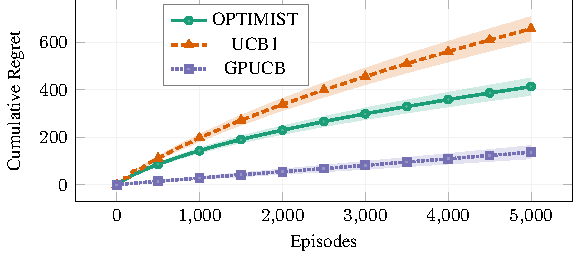
\includegraphics[width=\textwidth]{plots/lqg_mu/plot.pdf}
		\end{minipage}
		
		\textbf{River Swim} (Return)
		
		\begin{minipage}{.85\textwidth}
			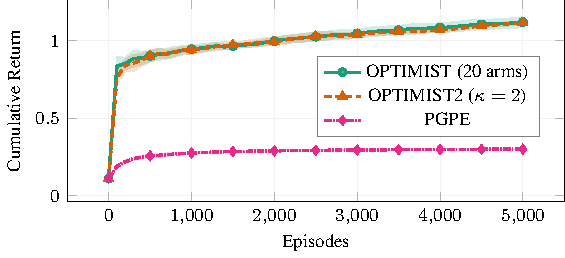
\includegraphics[width=\textwidth]{plots/riverswim/plot_main.pdf}
		\end{minipage}
		
		\textbf{Mountain Car} (Return)
		
		\begin{minipage}{.85\textwidth}
			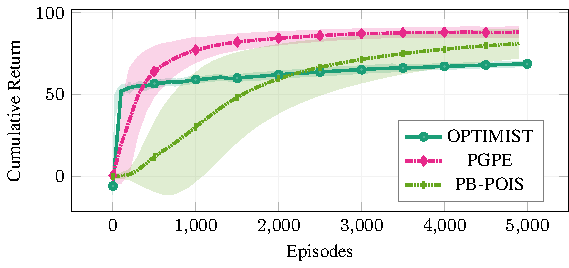
\includegraphics[width=\textwidth]{plots/mc/plot.pdf}
		\end{minipage}
	\end{center}

}

%%%%%%%%%%%%%%%%%%%%%%%%%%%%%%%%%%%%%%%%%%%%%%%%%%%%%%%%%%%%%%%%%%%%%%%%%%%%%%

%%%%%%%%%%%%%%%%%%%%%%%%%%%%%%%%%%%%%%%%%%%%%%%%%%%%%%%%%%%%%%%%%%%%%%%%%%%%%%

%%%%%%%%%%%%%%%%%%%%%%%%%%%%%%%%%%%%%%%%%%%%%%%%%%%%%%%%%%%%%%%%%%%%%%%%%%%%%%
\headerbox{References}{name=ref,column=3,row=2,span=1, below=exp, above=bottom}{
	%%%%%%%%%%%%%%%%%%%%%%%%%%%%%%%%%%%%%%%%%%%%%%%%%%%%%%%%%%%%%%%%%%%%%%%%%%%%%%
	\tiny
	\setlength{\bibsep}{0pt plus 0.3ex}
	\bibliographystyle{abbrvnat}
	\begingroup
	\renewcommand{\section}[2]{}%
	\bibliography{poster.bib}
	\endgroup
}

\end{poster}



\end{document}
